\chapter{Technique Overview}\label{ch:research}
The objective is to create an overview of techniques in the field.
According to the methodology detailed in~\ref{se:methodology}, first a taxonomy is introduced
which facilitates the analysis and comparison of techniques.
The subsequent search for literature which lays the foundation for an overview over current research
is documented.
Lastly, the advances in the field are placed in the correct position and analyzed.

\section{Pipeline taxonomy}\label{se:taxonomy}
Before getting into current research level, a base of knowledge about the field has to be layed.
\begin{table}[h]
    \centering\scriptsize
    \begin{tabular}{p{.04\textwidth}p{.11\textwidth}p{.16\textwidth}p{.55\textwidth}}
        Task & \multicolumn{2}{c}{Approach category} & Identifying properties \\
        \toprule
        STD & Seg free & & Localize whole instances, filter out false positives \\
            & & 1-stage & direct BB regression \\
            & & 2-stage & find ROIs, adjust ROIs for better fit \\
            & Seg based & & Localize sub text components to reconstruct instance \\
            & & Pixel-level & Pixel level segmentation \\
            & & Component-level & Sub-component level segmentation \\
        \midrule
        STR & Seg based & & Character segmentation and classification\\
            & \ac{EnDe} based & & Sequence recognition \\
            & & CTC based & CTC rule transciption \\
            & & Attention based & Attention Mechanism \\
        \midrule
        STS & 2 step & & Images are cropped for STR according to STD results \\
            & 2 stage & & Features are cropped for STR according to STD regions \\
        \bottomrule
    \end{tabular}
    \caption{Tasks, method categories and identifying propertis\label{tb:steps-properties}}
\end{table}
A taxonomy is created for this which is useful to classify and give context to innovations in the
field (see Table~\ref{tb:steps-properties}).
The partition of tasks and categorization of approaches is conducted according to overview literature
such as~\cite{long_scene_2021,chen_text_2021,cong_comparative_2019} and related research in the
field such as~\cite{qiao_text_2021,sheng_centripetaltext_2021,liu_accurate_2020,deng_pixellink_2018}.
Note that there can be approaches which blend different categories into one, the taxonomy
is merely used to facilitate an overview and to enable a clearer comparison.
In order to create the overview the necessary steps in the process of \ac{STS} need to be
highlighted, from localizing possible text instances to predicting the characters or
words~\citep{long_scene_2021, sourvanos_challenges_2018}.
Note that details which are not essential are abstracted away.
\ac{STD} and \ac{STR} only incorporate a part of \ac{STS}, while end to end approaches
incorporate both \ac{STD} and \ac{STR} techniques to solve
\ac{STS}~\citep{long_scene_2021,ghosh_visual_2017,chen_text_2021}.
Therefore this section will first discuss the two parts, to then later combine them.

\subsection{Scene Text Detection}
For \ac{STD} two main categories of approaches can be identified: segmentation based and \ac{BB}
regression based (see
Figure~\ref{fig:STD-pipelines})~\citep{long_scene_2021,sheng_centripetaltext_2021,liu_accurate_2020}.
\begin{figure}[ht]
    \centering
    \resizebox{0.6\linewidth}{!}{%
\begin{tikzpicture}[
    every node/.style={draw=black,thin,anchor=west, minimum height=2.5em},
    lroot/.style={%
        edge from parent fork down,
        level distance=0.5cm,
        text centered, text width=3cm},
    lone/.style={%
        text centered, text width=3cm,
        level distance=0.5cm},
    ltwo/.style={%
        text centered, text width=3cm,
        level distance=0.5cm},
    lthree/.style={%
        rounded corners,
        grow=down, xshift=-0.8cm,
        text centered, text width=3cm,
        edge from parent path={(\tikzparentnode.205) |- (\tikzchildnode.west)}},
    level1/.style ={level distance=1.2cm},
    level2/.style ={level distance=2.4cm},
    level3/.style ={level distance=3.6cm},
    level4/.style ={level distance=4.8cm},
    level5/.style ={level distance=6.0cm},
    level 1/.style={sibling distance=8cm},
    level 1/.append style={level distance=1.5cm},
    level 2/.style={sibling distance=4cm},
    level 2/.append style={level distance=1.5cm},
]
%   \draw[help lines] (0,0) grid (4,3);

    % lroot
    \node[anchor=south,lroot]{STD}
    [edge from parent fork down]
        child{node [lone] {BB regression}
            child{node [ltwo] {One-stage}
                child[lthree,level1] {node {Feature \\ extraction}}
                child[lthree,level2] {node {Text instance \\ localization}}
                child[lthree,level3] {node {Result \\ filtering}}
            }
            child{node [ltwo] {Two-stage}
                child[lthree,level1] {node {Feature \\ extraction}}
                child[lthree,level2] {node {Text region \\ localization}}
                child[lthree,level3] {node {Localization \\ readjustment}}
                child[lthree,level4] {node {Result \\ filtering}}
            }
        }
        child{node [lone] {Segmentation \\ based}
            child[lthree,level1] {node {Feature \\ extraction}}
            child[lthree,level2] {node {Sub-component \\ segmentation}}
            child[lthree,level3] {node {Text \\ reconstruction}}
        };
\end{tikzpicture}
}%

    \caption{Different STD pipelines\label{fig:STD-pipelines}}
\end{figure}
The regression based category draws heavy inspiration from the field of object
detection~\citep{long_scene_2021,liu_accurate_2020}.
This is only natural as text detection can be seen as a type of object
detection~\citep{liu_accurate_2020,long_scene_2021}.
For object detection inspired \ac{STD} there are two methods: one stage and two
stage~\citep{long_scene_2021}.
Both localize text instances as a whole in the form of a
\ac{BB} (see Figure~\ref{fig:STD-BB})~\citep{long_scene_2021,sheng_centripetaltext_2021}.
\begin{figure}[h]
    \centering
    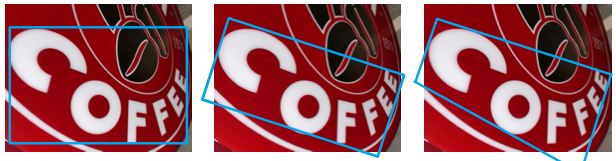
\includegraphics[width=0.7\textwidth]{img/STD-representation-BB-Liao-Textsnake-2018.png}
    \caption[Different bb text representation forms]{%
        Different bb text representation forms~\citep{ferrari_textsnake_2018}\label{fig:STD-BB}
    }
\end{figure}
One stage approaches are modelled after~\cite{liu_ssd_2016}, \ac{SSD} and~\cite{redmon_you_2016},
You Only Look Once (YOLO).
They have in comon that \acp{BB} are regressed once and not changed or optimized
afterwards~\citep{redmon_you_2016,liu_ssd_2016}, as opposed to the \ac{ROI} based approach with two
stages~\citep{girshick_rich_2014}.
The basic approach is explained with the example of~\cite{liao_textboxes_2017} (see
Figure~\ref{fig:STD-segfree-ssd}) which is based on \ac{SSD}.
\begin{figure}[ht]
    \centering
    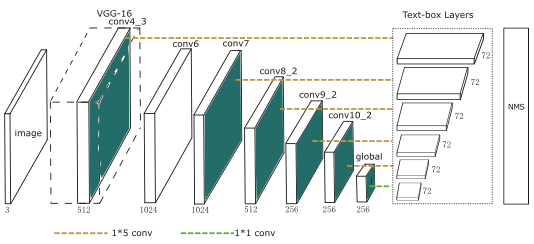
\includegraphics[width=0.8\textwidth]{img/STD-seg-free-Liao-TextBoxes-2017.png}
    \caption[One stage, BB regression based STD architecture]{%
        Example for a one stage, BB regression based STD
        architecture~\citep{liao_textboxes_2017}\label{fig:STD-segfree-ssd}
    }
\end{figure}
Note that the approach is modeled to recognize horizontal text instances~\citep{liao_textboxes_2017}.
It uses convolutional network inspired by the VGG architecture (blocks of: two or
three $3\times3$ conv layers followed by a $2\times2$ max pooling layer with stride 2) for feature
extraction~\citep{liao_textboxes_2017,simonyan_very_2015}.
Note that the spatial padding added for convolution ensures that spatial dimensions are
preserved~\citep{simonyan_very_2015}.
Afterwards come additional layers which continuously downsample.
The output of six of them is separately used as feature maps for \ac{BB}
regression~\citep{liao_textboxes_2017}.
The downsampling and \ac{BB} regression for different layers helps detect text instances of different
scales~\citep{liu_ssd_2016}.
Each spatial location on the feature map can be traced back to a region on the input
image~\citep{long_scene_2021}.
The \ac{BB} regression is carried out by six convolutional text-box layers which predict how
certain ($c_1,c_2$) the prediction is a text instance or background and where the text instance
is ($x,y,w,h$).
Note that the output is not the location of a \ac{BB} but the offset to the
respective anchor box~\citep{liao_textboxes_2017,long_scene_2021}.
Anchor boxes are predefined to give bias towards sizes and aspect ratios of
text~\citep{liao_textboxes_2017}.
The text-box layers are the difference to the \ac{SSD} approach for normal object
detection~\citep{liao_textboxes_2017,liu_ssd_2016}.
These layers use $1\times5$ filters to adjust to larger aspect ratios~\citep{liao_textboxes_2017}.
Each text-box layer has 72 filters (12 anchor boxes $\cdot$ 6 values per prediction), the filters
are slided accross the input features generating 12 predicted \ac{BB} per
position~\citep{liao_textboxes_2017}.
The \acp{BB} of all layers are then subjected to the process of \ac{NMS} to filter out the best
\ac{BB} for each possible text instance~\citep{liao_textboxes_2017}.
For this \ac{NMS} is used: of all detections which overlap (\ac{IOU}) more than a threshhold
$\phi$ only the with the highest confidence score ($c$) is kept~\citep{hosang_learning_2017}.

The R-CNN which builds the foundation for \ac{ROI} based text detection, was introduced
by~\cite{girshick_rich_2014} and improved by~\cite{girshick_fast_2015} (Fast
R-CNN),~\cite{ren_faster_2015} (Faster R-CNN) and~\cite{he_mask_2018} (Mask R-CNN).
Note that 2-stage methods are fully differentiable and thus end to end trainable since
Faster R-CNN (like 1-stage methods)~\citep{ren_faster_2015,long_scene_2021}.
The two stages consist of: \ac{ROI} regression, \ac{BB}
adjustments~\citep{jiang_r2cnn_2017, ren_faster_2015}.
The two stage \ac{STD} approach introduced by~\cite{jiang_r2cnn_2017} (see
Figure~\ref{fig:STD-segfree-rcnn}) uses Faster R-CNN.%
Unlike the previous approach, the architecture is designed to detect multi-oriented text
instances~\citep{jiang_r2cnn_2017,liao_textboxes_2017}.
\begin{figure}[ht]
    \centering
    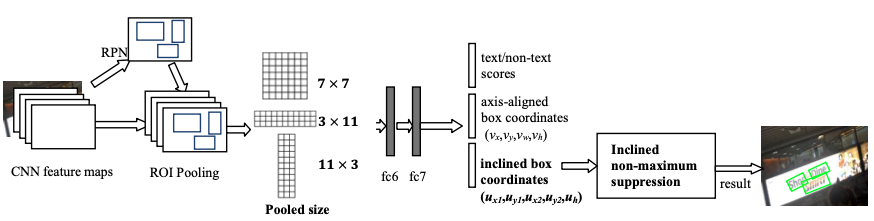
\includegraphics[width=0.8\textwidth]{img/STD-seg-free-Jiang-R2CNN-2017.png}
    \caption[Two stage, BB regression based STD architecture]{%
        Example for a two stage, BB regression based STD
        architecture~\citep{jiang_r2cnn_2017}\label{fig:STD-segfree-rcnn}
    }
\end{figure}
Like with the one stage approach, the two stage approach starts with feature extraction from the
image with a convolutional layers~\citep{jiang_r2cnn_2017}.
Feature extraction \ac{CNN} is again inspired by the VGG architecture~\citep{jiang_r2cnn_2017},
like in the previous approach.
The generated feature map is used by a \ac{RPN}.
Like with the previously explained approach, the feature maps are used to regress the offset
respective to \acp{BB}, however, these are considered as regions that probably contain text
that are subject to change and to be refined in a later
stage~\citep{jiang_r2cnn_2017,lu_mimicdet_2020}.
The \acp{BB} are still axis aligned at this point~\citep{jiang_r2cnn_2017}.
In contrast to the previous \ac{SSD} based approach, only one feature map is used in conjunction with
\ac{BB} regression~\citep{jiang_r2cnn_2017}.
The \ac{RPN} from Faster R-CNN is adjusted to use smaller scale anchor boxes to adapt to
text~\citep{jiang_r2cnn_2017}.
%Note that R-CNN and Fast-RCNN used the slower Sequential Search algorithm instead of an
%\ac{RPN}~\citep{girshick_rich_2014,girshick_fast_2015}.
The resulting \acp{BB} are called \acp{ROI}~\citep{ren_faster_2015,jiang_r2cnn_2017}.
They are used for \ac{ROI} pooling in conjunction with the original feature maps.
This layer uses max pooling to convert the spatial features corresponding to the location of the
\ac{ROI} to a small feature map~\citep{girshick_fast_2015}.
In the case of this example, \ac{ROI} pooling is used to create three feature maps with different
aspect ratios ($7\times7, 3\times11, 11\times3$) which are concatenated for the next
step~\citep{jiang_r2cnn_2017}.
The second stage is to predict a confidence score (text, background) for each \ac{ROI} and to
refine them by regressing values ($x_1,y_1,x_2,y_2,h$) that allow for multi-oriented boxes to account for
rotated text~\citep{jiang_r2cnn_2017}.
At last the resulting \acp{BB} are filtered by inclined \ac{NMS} which is adjusted to the
multi-oriented \acp{BB}~\citep{jiang_r2cnn_2017}.

The basis for the segmentation based methods is the fact that every part of the text instance can
be used to verify that there is text~\citep{long_scene_2021}.
Because of this, sub-text components can be detected separately and then used to re-construct a text
instance~\citep{long_scene_2021}.
Segmentation based methods can roughly be summed up in two categories: pixel level and component
level~\citep{long_scene_2021}.
Like with \ac{BB} regression based methods, example architectures are explained in order to
describe their categories more clearly.
The first segmentation based category for \ac{STD} segments components which are local regions of
text that can overlap one or more characters~\citep{long_scene_2021}.
\begin{figure}[ht]
    \centering
    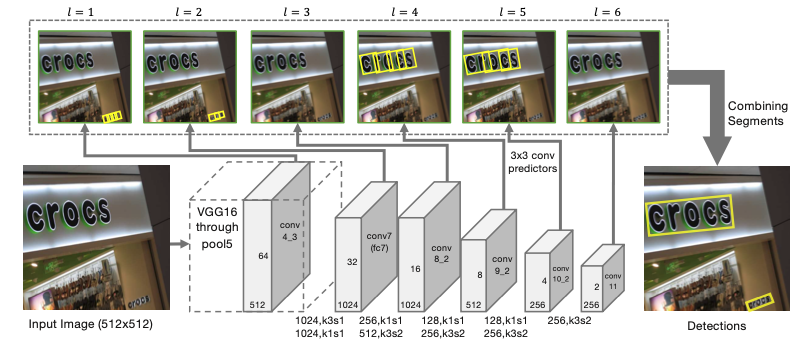
\includegraphics[width=0.9\textwidth]{img/STD-seg-based-architecture-Shi-Detecting-2017.png}
    \caption[Sub-component, segmentation based STD architecture]{%
        Example for a sub-component, segmentation based STD
        architecture~\citep{shi_detecting_2017}\label{fig:STD-segbased-component-architecture}
    }
\end{figure}
The architecture (see Figure~\ref{fig:STD-segbased-component-architecture})
from~\cite{shi_detecting_2017} is used as an example for this category.
Like the one-stage, \ac{BB} regression based \ac{STD} approach, the feature extraction \ac{CNN} of
this approach is taken from \ac{SSD} and thus VGG, the difference is reflected in the prediction
layers~\citep{shi_detecting_2017,liu_ssd_2016,simonyan_very_2015}.
Instead of detecting whole \acp{BB}, the networks predicts both subcomponents and links at multiple
scales~\citep{shi_detecting_2017}.
The convolutional prediction is carried out with seven $3\times3$ filters followed by a \sfmx\
nonlinearity for normalization.
The segments are given by the values $x_s,y_s,w_s,h_s,\theta_s$ which offset an anchor box as well
as confidence scores $c_1,c_2$~\citep{shi_detecting_2017}.
Links ($s_1,s_2$) are used to combine the segments and are accordingly used to separate neraby
words~\citep{shi_detecting_2017}.
\begin{figure}[ht]
    \centering
    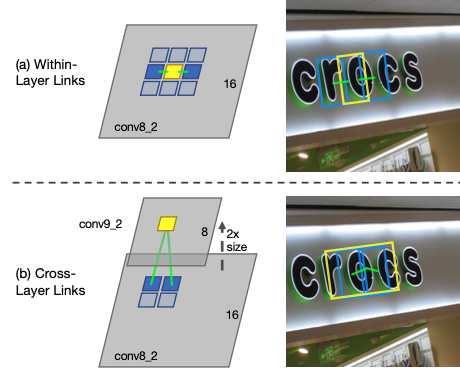
\includegraphics[width=0.5\textwidth]{img/STD-seg-based-links-Shi-Detecting-2017.png}
    \caption[Predicting links for segmentation based STD]{%
        Visualization for prediction of links within and cross layers for segmentation based
        STD~\citep{shi_detecting_2017}\label{fig:STD-segbased-component-links}
    }
\end{figure}
The convolutional link predictions are then used to as follows:
Within layer links are for the neighbors of a space in the predicted feature map
(see Figure~\ref{fig:STD-segbased-component-links} (a),
Equation~\ref{eq:STD-segbased-subcomp-same-layer})~\citep{shi_detecting_2017}.
\begin{equation}\label{eq:STD-segbased-subcomp-same-layer}
    \mathcal{N}_{s^{x,y,l}}^w =
        \frac{{\{s^{(x',y',l)}\}}_{x-1\leq x'\leq x+1,y-1\leq y'\leq y+1}}{s^{(x,y,l)}}
\end{equation}
The cross layer links on the other hand are found by using the 4 cross layer neighors of the
feature map of the preceding predictor~\citep{shi_detecting_2017}.
(see Figure~\ref{fig:STD-segbased-component-links} (b),
Equation~\ref{eq:STD-segbased-subcomp-cross-layer})~\citep{shi_detecting_2017}.
\begin{equation}\label{eq:STD-segbased-subcomp-cross-layer}
    \mathcal{N}_{s^{x,y,l}}^c = {\{s^{(x',y',l-1)}\}}_{2x\leq x'\leq 2x+1,2y\leq y'\leq 2y+1}
\end{equation}
These cross layer links are used to connect segments on different scales~\citep{shi_detecting_2017}.
The network architecture designed so that the preceding feature map is twice the size (spatial
dimensions) of the current which is necessary to extract the right
locations~\citep{shi_detecting_2017}.
Before reconstruction the text instances, segments are filtered by their confidence
scores~\citep{shi_detecting_2017}.
To reconstruct, the predictions are taken as a graph: segments are nodes, links are edges.
Depth-first search is applied to the graph to find connected components and thus text
instances~\citep{shi_detecting_2017}.

The paper~\cite{deng_pixellink_2018} introduced a pixel level \ac{STD} approach.
It adapts the previous component level \ac{STD} approach to work on pixel
level~\citep{deng_pixellink_2018}.
\begin{figure}[ht]
    \centering
    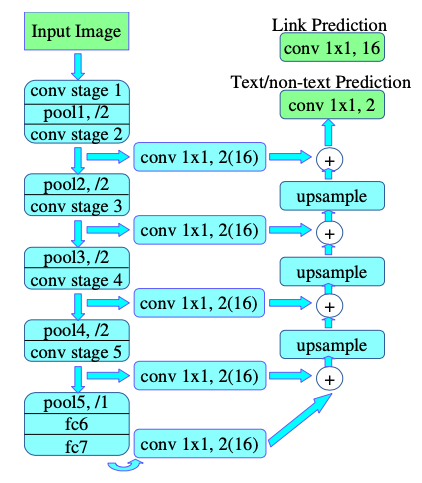
\includegraphics[width=0.35\textwidth]{img/STD-seg-based-CNN-Deng-PixelLink-2018.png}
    \caption[Feature extractor and prediction head for pixel segmentation]{%
        PixelNet CNN feature extractor with head structure for pixel
        segmentation\label{fig:STD-segbased-pixel-CNN}
    }
\end{figure}
Figure~\ref{fig:STD-segbased-pixel-CNN} shows the \ac{CNN} structure for feature extraction
(until conv5) which is basically VGG architecture with the fully connected layers exchanged with
another convolutional stage~\citep{deng_pixellink_2018}.
Inspired by~\cite{long_fully_2015}, the structure then combines downsampled feature maps with later
upsampled ones~\citep{deng_pixellink_2018}.
Pixel level segmentation approaches mostly rely on \acp{FCN}~\citep{dai_fused_2018}.
Continuous downsampling and and combining those layers with later, upsampled layers helps
to combine coarse, higher level information with fine, lower level
information~\citep{long_fully_2015}.
The upsampling is performed with bilinear interpolation~\citep{deng_pixellink_2018}.
The feature extraction is followed by two heads which either predict text/non-text or
links~\citep{deng_pixellink_2018}.
This creates dense segmentation maps which are used to then segregate different
instances of text~\citep{deng_pixellink_2018}.
Depending on which head is used, the $1\times1$ convolution layers either have 2 or $2\cdot8$ filters.
Counted together, the model has 18 output channels~\citep{deng_pixellink_2018}.
2 filters are used to predict text/non-text for each pixel, while the other 16 filters predict
the links~\citep{deng_pixellink_2018}.
The text/non-text head essentially performs semantic segmentation, that is to categorize each
pixel to its object type~\citep{deng_pixellink_2018}.
For every neighbor there is a negative and a positive score.
A pixel has eight neighbors: left, left-down, left-up, right, right-down, right-up, up, down.
Each of the $2\cdot8$ filters is responsible for a neighbor link~\citep{deng_pixellink_2018}.
\begin{figure}[hb]
    \centering
    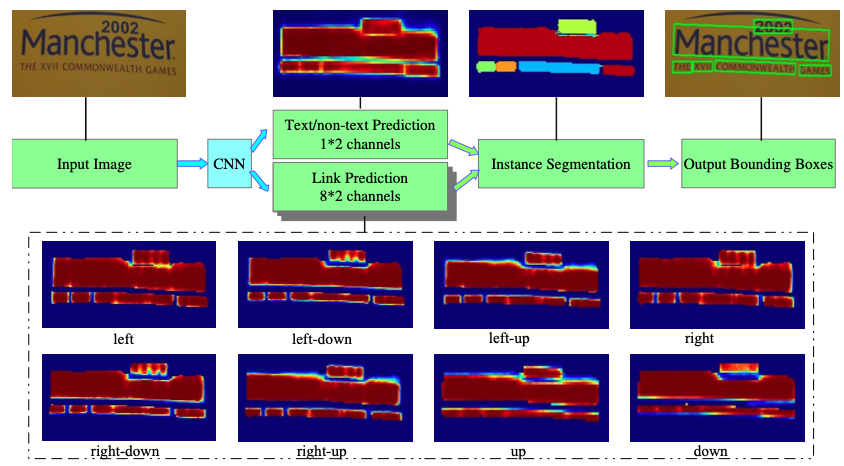
\includegraphics[width=0.7\textwidth]{img/STD-seg-based-architecture-Deng-PixelLink-2018.png}
    \caption[Pixel, segmentation based STD architecture]{%
        Example for a pixel, segmentation based STD
        architecture~\citep{deng_pixellink_2018}\label{fig:STD-segbased-pixel-architecture}
    }
\end{figure}
After both links and text/non-text pixels have been predicted, they are combined for instance
segmentation~\citep{deng_pixellink_2018}.
The link layers are used to indicate whether two text pixels are grouped together an thus belong to
the same instance~\citep{deng_pixellink_2018}.
The output is a dense prediction map with the same spatial structure as the input
image~\citep{deng_pixellink_2018}.
A bounding box can then be extracted by laying minimum area rectangles over the
instances~\citep{deng_pixellink_2018}.
Figure~\ref{fig:STD-segbased-pixel-architecture} shows the whole pipeline.


\subsection{Scene Text Recognition}
For \ac{STR} two main categories of approaches can be identified: segmentation based and
\ac{EnDe} based (see Figure~\ref{fig:str-pipelines})~\citep{chen_text_2021}.
\begin{figure}[h]
    \centering
    \resizebox{0.6\linewidth}{!}{%
\begin{tikzpicture}[
    every node/.style={draw=black,thin,anchor=west, minimum height=2.5em},
    lroot/.style={%
        edge from parent fork down,
        level distance=0.5cm,
        text centered, text width=3cm},
    lone/.style={%
        text centered, text width=3cm,
        level distance=0.5cm},
    ltwo/.style={%
        text centered, text width=3cm,
        level distance=0.5cm},
    lthree/.style={%
        rounded corners,
        grow=down, xshift=-0.8cm,
        text centered, text width=3cm,
        edge from parent path={(\tikzparentnode.205) |- (\tikzchildnode.west)}},
    level1/.style ={level distance=1.2cm},
    level2/.style ={level distance=2.4cm},
    level3/.style ={level distance=3.6cm},
    level4/.style ={level distance=4.8cm},
    level5/.style ={level distance=6.0cm},
    level 1/.style={sibling distance=6cm},
    level 1/.append style={level distance=1.5cm},
    level 2/.style={sibling distance=5cm},
    level 2/.append style={level distance=1.5cm},
]
%   \draw[help lines] (0,0) grid (4,3);

    % lroot
    \node[anchor=south,lroot]{STR}
    [edge from parent fork down]
        child{node [ltwo] {Segmentation \\ based}
            child[lthree,level1] {node {Image \\ preprocessing}}
            child[lthree,level2] {node {Feature \\ extraction}}
            child[lthree,level3] {node {Character \\ segmentation}}
            child[lthree,level4] {node {Character \\ recognition}}
        }
        child{node [lone] {Segmentation \\ free}
            child{node [ltwo] {CTC}
                child[lthree,level1] {node {Image \\ preprocessing}}
                child[lthree,level2] {node {Feature \\ extraction}}
                child[lthree,level3] {node {Sequence \\ modelling}}
                child[lthree,level4] {node {CTC rule \\ application}}
            }
            child{node [ltwo] {Encoder-Decoder}
                child[lthree,level1] {node {Image \\ preprocessing}}
                child[lthree,level2] {node {Feature \\ extraction}}
                child[lthree,level3] {node {Sequence \\ modelling}}
                child[lthree,level4] {node {Sequence \\ decoder}}
            }
        };
\end{tikzpicture}
}%

    \caption{Different STR pipelines\label{fig:str-pipelines}}
\end{figure}
Segmentation based approaches for \ac{STR} are similar to segmentation based approaches for \ac{STD}.
After feature extraction, the subtext components (characters for \ac{STR}) are
segmented~\citep{chen_text_2021}.
Instead of reconstructing a \ac{BB}, the characters are classified to recognize the
text and are then used to form the text instance~\citep{chen_text_2021}.
Because of their similarity to \ac{STD} and the recent domiance of \ac{EnDe} based
approaches~\citep{chen_text_2021,long_scene_2021}, only the later will be explained in detail with
examples.
\begin{figure}[hb]
    \centering
    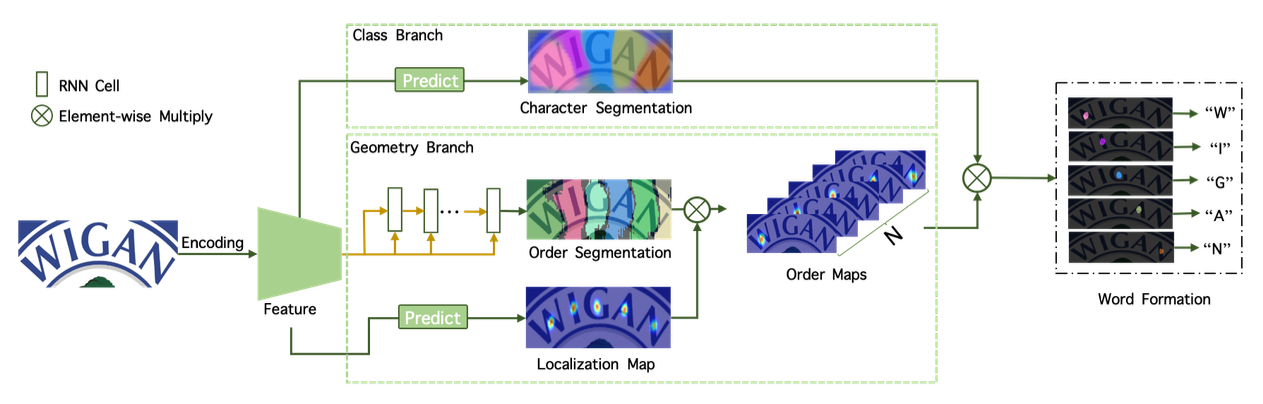
\includegraphics[width=0.8\textwidth]{img/STR-seg-based-wan-textscaner-2020.png}
    \caption[Segmentation based STR architecture]{%
        Example for segmentation based STR
        architecture~\citep{wan_textscanner_2020}\label{fig:STR-segbased-architecture}
    }
\end{figure}
The approach from~\cite{wan_textscanner_2020} can be used as an example, should the reader feel the
need to read up on segmentation based methods for \ac{STR} that do not include an \ac{EnDe}
mechanism in the prediciton stage.
The approach adds a geometry branch parallel to the charcater segmentation which helps with with
putting the identified characters in the right sequence (see
Figure~\ref{fig:STR-segbased-architecture})~\citep{wan_textscanner_2020}.

For \ac{EnDe} based \ac{STR} there are twomein categories: \ac{CTC} based and attention
based~\citep{chen_text_2021}.
These two categories can be distinguished by the way the decoder works~\citep{chen_text_2021}.
The previous stages in the pipeline are similar~\citep{long_scene_2021,chen_text_2021}.
Often preprocessing stages are performed to remove distortions, rectify curved text,
remove disruptive background, improve resolutions or recover degraded text.
Especially rectifying curved text (see Figure~\ref{fig:STN-application}) with the help of
thin-plate spines~\citep{bookstein_principal_1989} and spatial transformer
networks~\citep{jaderberg_spatial_2015} shows great improvement for \ac{STR}
performance~\citep{long_scene_2021,chen_text_2021}.
\begin{figure}[h]
    \centering
    
\includegraphics[width=0.4\textwidth]{img/STN-result-Liu-STAR-2016.png}
    \caption[Text rectification application]{%
        Application of spatial transformer network to rectify curved
        text~\citep{liu_star-net_2016}\label{fig:STN-application}
    }
\end{figure}
For feature extraction different \ac{CNN} architectures can be chosen.
The tradeoff between performance and memory \& computation cost determines what \ac{CNN} should be
chosen~\citep{chen_text_2021}.
An example for a deep and powerful \ac{CNN} are ResNets~\citep{he_deep_2015} which are often used
for benchmark purposes~\citep{chen_text_2021,long_scene_2021}.
Refer to Section~\ref{se:cnn} for more information on ResNets.
Efficient feature extraction can e.g.\ be performed with binary convolutional
nets~\citep{liu_squeezedtext_2018}.
For the sequence modelling and transcription steps first~\cite{shi_end--end_2017} (\ac{CTC} based)
and then~\cite{ghosh_visual_2017} (attention based) will be used as examples.
\begin{figure}[h]
    \centering
    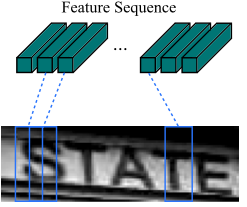
\includegraphics[width=0.3\textwidth]{img/STR-encdec-sequence-feat.png}
    \caption[Sequential feature extraction from convolution feature maps]{%
        Sequential feature extraction from convolution feature
        maps~\citep{shi_end--end_2017}\label{fig:STR-CTC-seq-feat}
    }
\end{figure}
For~\cite{shi_end--end_2017} the sequence is generated by taking column out of the feature maps
from left to right (see Figure~\ref{fig:STR-CTC-seq-feat})~\citep{shi_end--end_2017}.
This is possible because the parts of the feature map correspond to a spatial region of the
original image~\citep{shi_end--end_2017,goodfellow_deep_2016}.
This encoding corresponds to a 1d representation that neglects vertical spatial
information~\citep{cong_comparative_2019}.
The generated sequence features are feed into a deep \ac{BiLSTM}.
Figure~\ref{fig:bilstm} shows one layer which is made up of an \ac{LSTM} which processes the
sequence in the correct order and another \ac{LSTM} which processes the sequence
backwards~\citep{shi_end--end_2017}.
An \ac{LSTM} processed a sequence to gather context from ealier input for laterr
outputs~\citep{shi_end--end_2017,goodfellow_deep_2016}.
The \ac{BiLSTM} allows to gather context of later input for ealier outputs~\citep{shi_end--end_2017}.
This is important since a character might comprise more than one step in the sequence
data~\citep{shi_end--end_2017}.
\begin{figure}[ht]
    \centering
    {\scriptsize%
\begin{tikzpicture}[scale=0.3]
	\node[rectangle] (Y0) at (0, 0) {$\dots$};
	\node[rectangle, draw, right=2em of Y0, minimum height=1cm, minimum width=1cm] (RNN)
        {LSTM$_\rightarrow$};
	\node[rectangle, right=of RNN, draw, minimum height=1cm, minimum width=1cm] (RNN2)
        {LSTM$_\rightarrow$};
	\node[rectangle, right=of RNN2, draw, minimum height=1cm, minimum width=1cm] (RNN3)
        {LSTM$_\rightarrow$};
	\node[rectangle, right= of RNN3, draw, minimum height=1cm, minimum width=1cm] (RNN4)
        {LSTM$_\rightarrow$};
	\node[rectangle, right=2em of RNN4] (RNN5) {$\dots$};


	\node[rectangle, above=of RNN4, draw, minimum height=1cm, minimum width=1cm] (R25)
        {LSTM$_\leftarrow$};
	\node[rectangle, left=of R25, minimum height=1cm, minimum width=1cm, draw] (R24)
        {LSTM$_\leftarrow$};
	\node[rectangle, left=of R24, draw, minimum height=1cm, minimum width=1cm] (R23)
        {LSTM$_\leftarrow$};
	\node[rectangle, left=of R23, draw, minimum height=1cm, minimum width=1cm] (R22)
        {LSTM$_\leftarrow$};
	\node[rectangle, left=2em of R22] (R21) {$\dots$};
	\node[right=2em of R25] (Y20) {$\dots$};

	\node[below=of RNN] (X1) {$\x_2$};
	\node[below=of RNN2] (X2) {$\x_3$};
	\node[below=of RNN3] (X3) {$\x_4$};
	\node[below=of RNN4] (X4) {$\x_5$};
	\node[above=of R25] (Y5) {$\h_5$};
	\node[above=of R24] (Y4) {$\h_4$};
	\node[above=of R23] (Y3) {$\h_3$};
	\node[above=of R22] (Y2) {$\h_2$};
	\node[rectangle, left=3.2em of Y2] (Y1) {$\dots$};
	\node[right=3.2em of Y5] (Y6) {$\dots$};

	\draw[-stealth] (X1) -- (RNN);
	\draw[-stealth] (X2) -- (RNN2);
	\draw[-stealth] (X3) -- (RNN3);
	\draw[-stealth] (X4) -- (RNN4);
	\draw[-stealth, densely dotted] (Y0) -- (RNN);
	\draw[-stealth] (RNN) -- node[above, pos=0.35] {} (RNN2);
	\draw[-stealth] (RNN2) -- node[above, pos=0.35] {} (RNN3);
	\draw[-stealth] (RNN3) -- node[above, pos=0.35] {} (RNN4);
	\draw[-stealth, densely dotted] (RNN4) -- (RNN5);
	\node[below=4em of Y0] (d) {\dots};
	\node[below=4em of RNN5] (d) {\dots};

	\path[-stealth, white] (X1) edge[bend left=45] (R22);
	\path[-stealth] (X1) edge[bend left=45] (R22);
	\path[-stealth, white] (X2) edge[bend left=45] (R23);
	\path[-stealth] (X2) edge[bend left=45] (R23);
	\path[-stealth, white] (X3) edge[bend left=45] (R24);
	\path[-stealth] (X3) edge[bend left=45] (R24);
	\path[-stealth, white] (X4) edge[bend left=45] (R25);
	\path[-stealth] (X4) edge[bend left=45] (R25);
	\draw[-stealth, densely dotted] (Y20) -- (R25);

	\draw[-stealth] (R22) -- (Y2);
	\draw[-stealth] (R23) -- (Y3);
	\draw[-stealth] (R24) -- (Y4);
	\draw[-stealth] (R25) -- (Y5);

	\draw[stealth-, densely dotted] (R21) -- (R22);
	\draw[stealth-] (R22) -- node[above, pos=0.65] {} (R23);
	\draw[stealth-] (R23) -- node[above, pos=0.65] {} (R24);
	\draw[stealth-] (R24) -- node[above, pos=0.65] {} (R25);
	\draw[-stealth, densely dotted] (Y20) -- (R25);

	\path[-stealth, white] (RNN) edge[bend right=45] (Y2);
	\path[-stealth] (RNN) edge[bend right=45] (Y2);
	\path[-stealth, white] (RNN2) edge[bend right=45] (Y3);
	\path[-stealth] (RNN2) edge[bend right=45] (Y3);
	\path[-stealth, white] (RNN3) edge[bend right=45] (Y4);
	\path[-stealth] (RNN3) edge[bend right=45] (Y4);
	\path[-stealth, white] (RNN4) edge[bend right=45] (Y5);
	\path[-stealth] (RNN4) edge[bend right=45] (Y5);
\end{tikzpicture}
}
%
    \caption[Bidirectional LSTM]{%
        Bidirectional LSTM~\citep{goodfellow_deep_2016}\label{fig:bilstm}
    }
\end{figure}
The generated encoded features with embedded context are then used for transcribing the final
output~\citep{shi_end--end_2017}.
The transciption uses conditional probibilities to convert the per-frame features encoded by the
deep \ac{BiLSTM} into the label sequence which is the text instance
prediction~\citep{shi_end--end_2017}.
This process uses the conditional probabilities $p(l\|\Y)$ that are defined
by~\cite{graves_connectionist_2006}, which is why the category of approaches is called
\ac{CTC} based.
$l$ stands for the predicted character sequence and \Y\ stands for the per-frame
features~\citep{shi_end--end_2017}.
Each frame $\y_t$ is a probability distribution over the possible character and a `blank'
character~\citep{shi_end--end_2017,graves_connectionist_2006}.
It is distinguished between lexicon based and lexicon free transcription~\citep{shi_end--end_2017}.
Lexicon free transcription uses the most probable character or blank (-) at each frame.
\[\text{HHH-eellll-lll-\-oo-\-\-}\]
Then all duplicate characters are discarded.
\[\text{H-el-l-o}\]
At last all blanks are discarded, leaving the final prediction~\citep{shi_end--end_2017}.
\[\text{Hello}\]
For lexicon based transcription the combination of \Y\ is checked for similarity to words in the
lexicon based on the levenstein distance (like the metrics \ac{AED}, \ac{NED} defined in
Section~\ref{se:sts})~\citep{shi_end--end_2017}.
The process of searching for similarity can be efficiently implemented with the BK-tree data
structure~\citep{burkhard_approaches_1973,shi_end--end_2017}.
The word in the lexicon with the largest probability to be derived from \Y\ is
chosen~\citep{shi_end--end_2017}.

For an attention based example, the approach introduced by~\cite{ghosh_visual_2017} is used.
The approach is inspired by~\cite{bahdanau_neural_2016,xu_show_2016}: It uses a \ac{CNN} for
spatial encoding of the input image which can then be used.
The attention mechanism then helps the subsequent \ac{LSTM} to choose part of the image most
important for each timestep~\citep{ghosh_visual_2017}.
\begin{figure}[h]
    \centering
    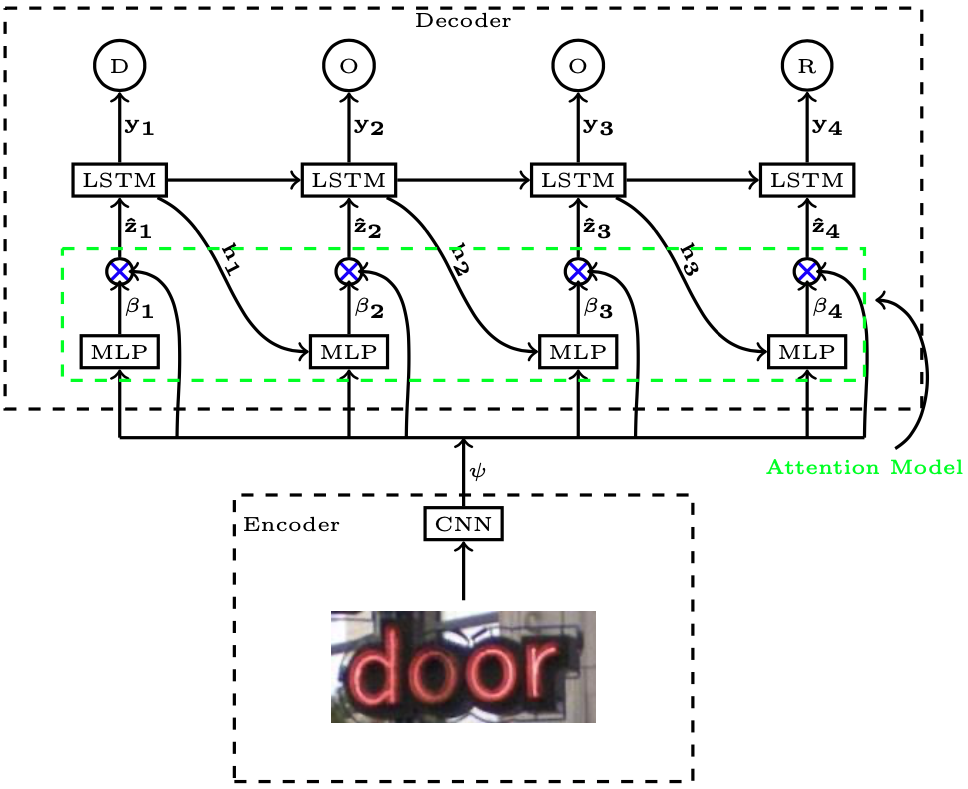
\includegraphics[width=0.7\textwidth]{img/STR-encdec-attention-Gosh-Visual-2017.png}
    \caption[Encoder decoder \& attention based STR architecture]{%
        Encoder decoder based STR architecture with attention
        mechanism~\citep{ghosh_visual_2017}\label{fig:STR-attention}
    }
\end{figure}
Figure~\ref{fig:STR-attention} shows the network architecture~\citep{ghosh_visual_2017}.
The \ac{CNN} performs feature extraction~\citep{ghosh_visual_2017}.
The feature map is then encoded into feature vectors like in
Figure~\ref{fig:STR-CTC-seq-feat}~\citep{ghosh_visual_2017,shi_end--end_2017}.
The attention mechanism is placed between the encoder \ac{CNN} and the decoder
\ac{LSTM}~\citep{ghosh_visual_2017}.
Note that some approaches consider the attention mechanism to be a part of the
decoder~\citep{shi_aster_2019}.
This mechanism uses a weighted combination of the \sfmx\ activation ($\boldsymbol{\beta}_{t,i}$) of
the \ac{MLP} output ($\Phi$) and the feature vectors to encode the relative importance of the
image parts at each time step (see Equations~\ref{eq:attention-weighted-combination}
and~\ref{eq:attention-gate-values})~\citep{ghosh_visual_2017,xu_show_2016}.
\begin{equation}\label{eq:attention-weighted-combination}
    \hat{\textbf{z}}_t=\sum_{i=1}^{K}\boldsymbol{\beta}_{t,i}\cdot \x_i
\end{equation}
\begin{equation}\label{eq:attention-gate-values}
    \boldsymbol{\beta}_{t}=\sfmx(\Phi(\x_i,\h_{t-1}))
\end{equation}
Like with the previous approach, the networks output vectors at each time step represent a
probability distribution over all possible characters~\citep{ghosh_visual_2017}.
The transciption process again has the option to be used with a lexicon and
without~\citep{ghosh_visual_2017}.
The basic process without a lexicon leverages the beam search algorithm~\citep{ghosh_visual_2017}
to find the sequence $w=[c_1,c_2,\ldots,c_n]$ with the highest
probability~\citep{ghosh_visual_2017}.
For lexicons the beam search algorithm is adjusted so that any sequences that that do not belong
to a word in the lexicon fall out of contention~\citep{ghosh_visual_2017}.
Besides the possibility to use a lexicon, the approach can also incorporate language priors into
the beam search process.
These priors leverage knowledge about the language that is recognized~\citep{ghosh_visual_2017}.

\subsection{Scene Text Spotting}
As mentioned, \ac{STD} and \ac{STR} are only parts of the task that is at the center of this thesis.
\ac{STS} can be performed in two ways (see Figure~\ref{fig:e2e-pipelines}).
\begin{comment}
\begin{figure}[ht]
    \centering
    \subfigure[2 step pipeline consisting of separate STD and STR\label{fig:e2e-2-step}]{%
        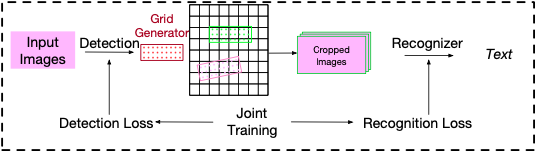
\includegraphics[width=0.65\textwidth]{img/E2E-2-step-Long-Scene-2021.png}
    }
    \subfigure[2 stage pipeline consisting of one joint architecture for STS\label{fig:e2e-2-stage}]{%
        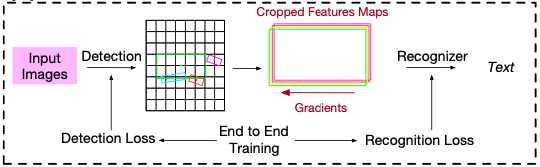
\includegraphics[width=0.65\textwidth]{img/E2E-2-stage-Long-Scene-2021.png}
    }
    \caption[Different end to end pipelines for STS]{%
        Different end to end pipelines for STS~\citep{long_scene_2021}\label{fig:looooong}
    }
\end{figure}
\end{comment}
\begin{figure}[ht]
    \centering
    \resizebox{0.4\linewidth}{!}{%
\begin{tikzpicture}[
    every node/.style={draw=black,thin,anchor=west, minimum height=2.5em},
    lroot/.style={%
        edge from parent fork down,
        level distance=0.5cm,
        text centered, text width=3cm},
    lone/.style={%
        text centered, text width=3cm,
        level distance=0.5cm},
    ltwo/.style={%
        rounded corners,
        grow=down, xshift=-0.8cm,
        text centered, text width=3cm,
        edge from parent path={(\tikzparentnode.205) |- (\tikzchildnode.west)}},
    level1/.style ={level distance=1.2cm},
    level2/.style ={level distance=2.4cm},
    level3/.style ={level distance=3.6cm},
    level4/.style ={level distance=4.8cm},
    level5/.style ={level distance=6.0cm},
    level 1/.style={sibling distance=4cm},
    level 1/.append style={level distance=1.5cm},
]
%   \draw[help lines] (0,0) grid (4,3);

    % lroot
    \node[anchor=south,lroot]{E2E}
    [edge from parent fork down]
            child{node [lone] {2-step}
                child[ltwo,level1] {node {STD \\ }}
                child[ltwo,level2] {node {STR with \\ cropped images}}
            }
            child{node [lone] {2-stage}
                child[ltwo,level1] {node {STD}}
                child[ltwo,level2] {node {STR with \\ feature maps}}
            };
        %

\end{tikzpicture}
}%

    \caption{Different STS pipelines\label{fig:e2e-pipelines}}
\end{figure}
(1) Run \ac{STD}, crop the image at the resulting bounding boxes, run \ac{STR}.
(2) Run \ac{STD}, crop feature maps, run adjusted \ac{STR}~\citep{chen_text_2021,long_scene_2021}.
Two step methods can modularly be combined~\citep{liao_textboxes_2017,shi_aster_2019}.
The \ac{STD} approach from~\cite{liao_textboxes_2017} can be combined with the CTC based \ac{STR}
from~\cite{shi_end--end_2017}.
Note that for the two step modular approaches can still be adjusted to better fit
together~\citep{liao_textboxes_2017}.
The two stage approach that is used as an example was introduced by~\cite{busta_deep_2017}.
\begin{figure}[h]
    \centering
    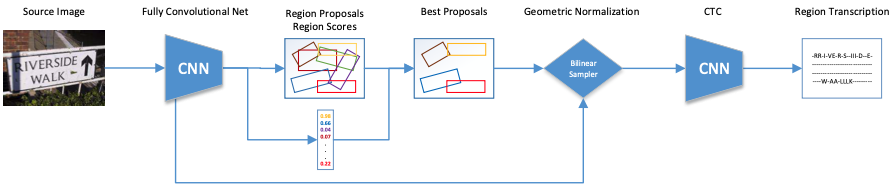
\includegraphics[width=0.95\textwidth]{img/E2E-two-stage-architecture-Bust-Deep-2017.png}
    \caption[2 stage STS architecture]{%
        2 stage STS architecture~\citep{busta_deep_2017}\label{fig:e2e-2-stage}
    }
\end{figure}
The approach essentially combines \ac{BB} based \ac{ROI} \ac{STD} with \ac{EnDe} based \ac{CTC}
\ac{STR}.
After extracting features with a \ac{CNN}, the approach first generates \acp{ROI}.
All \acp{ROI} with a certainty score above a threshhold are passed over to the recognition
module~\citep{busta_deep_2017}.
The combination of detection and recognition is made possible by bilinear
sampling~\citep{busta_deep_2017}.
This technique helps to collect the correct spatial features in terms of placing, size and rotation
to pass to the recognition part~\citep{busta_deep_2017}.
Note that the transformation normalized the rotation of the \acp{ROI}~\citep{busta_deep_2017}.
At this point \acp{ROI} with a confidence score under a threshhold are
discarded~\citep{busta_deep_2017}.
Sampling is the process of selecting the right spatial features from the respective \ac{ROI} area
that can be used for recognition~\citep{liu_abcnet_2020}.
The transformed \ac{ROI} features are then processed by a \ac{CNN} which transforms the feature maps
into one feature map whose height is defined by the predictable characters and the width is defined
by the spatial features of the \ac{ROI}~\citep{busta_deep_2017}.
The resulting values can be tranformed into \ac{CTC} probability
distributions~\citep{busta_deep_2017,graves_connectionist_2006}.
Then the \ac{CTC} transcription rule can be applied to generate the final result.
As with normal \ac{ROI} based approaches, a text instances can be mapped to multiple
predictions~\citep{ren_faster_2016,busta_deep_2017}.
Instead of performing \ac{NMS} with the help of the certainty score of \acp{ROI}, the filtering
is performed with certainty scores which are generated in the recognition phase of the
model~\citep{busta_deep_2017}.

\section{State of the Art Methods}\label{se:innovations}
This section documents the search for literature which provides the content for the subsequent
overview of innovation.
For this, important \ac{DL} techniques and notable advances along with their properties are researched
and presented.
Note that not the whole approaches that are introduced are explained, but only the innovation that
improves upon previous work.
For a literature review, it is important to report how the information was found and
synthesized~\citep{torraco_writing_2005}.
The strategy for researching current research is most important for a literature
review~\citep{snyder_literature_2019}.
This includes databases and keywords that were used, as well as exclusion criteria that were
enforced~\citep{torraco_writing_2005}.

The literature is identified through searching in the Google Scholar database.
The search is executed with keywords such as, but not only: Scene Text Detection,
Scene Text Recognition, Scene Text Spotting.
For identified literature, the citations are investigated to find further innovations in the field.
A criterion for examination is an appropriate amount of citations ($>100$) for the piece of
literature in question.
This cutoff point is defined to filter the most influential research.
All research after 2018 which pertains innovations for model architecture for extracting scene
text is regarded as relevant.
Standard \ac{OCR} solutions may not hold validity in practice, as the image and text conditions can
vary in the defined problem~\citep{chen_text_2021}.
The delimination from Section~\ref{se:problem} of course holds for this chapter and only literature
which concerns advances for the \ac{DL} model architecture will be regarded as important for the
scope of this thesis.
This extends to the whole pipeline from extracting features to the final result of the model.

\subsection{Detection Innovations}
\begin{table}[ht]
    \centering\scriptsize
    \begin{tabular}{p{.09\textwidth}p{.158\textwidth}p{.198\textwidth}p{.03\textwidth}
            p{0.27\textwidth}p{0.05\textwidth}p{0.05\textwidth}}
    \multicolumn{2}{c}{\textbf{Approach category}} & \textbf{Source} & \textbf{\#cit} &
    \textbf{Innovation} & \textbf{Orien-tation} & \textbf{Improve-ment} \\
        \toprule
        Seg free & & \\
            & 1-stage &~\cite{liao_textboxes_2018} & 499 & Multi-oriented BBs with
                new quadrilateral representation & m & e\\
            & &~\cite{liao_rotation-sensitive_2018} & 300 & Rotation sensitive features
                for BBs and insensitive features for text certainty & m & p\\
            & 2-stage &~\cite{ma_arbitrary-oriented_2018} & 724 & Rotation RPN and rotated \ac{ROI}
                pooling & m & p\\
        \midrule
        Seg based & & \\
            & Pixel-level &~\cite{deng_pixellink_2018} & 402 & Combine text with neighbor predictions for
                reconstruction & m & p\\
            & &~\cite{lyu_multi-oriented_2018} & 263 & Combine corner localization w\ position sensitive
                segmentation & m & e \\
            & &~\cite{liao_real-time_2019} & 160 & Differential binarization for
                reconstruction  & c & e \\
            & &~\cite{wang_efficient_2019} & 122 & Efficient segmentation with lightweight feature
                extractor & c & e \\
            & &~\cite{xu_textfield_2019} & 155 & Directions away
                from nearest boundary for textfield representation & c & p \\
            & &~\cite{wang_shape_2019} & 266 & Multiple segmentation maps at different scales
                & c & p\\
            & &~\cite{ferrari_textsnake_2018} & 301 & Representation based on
                a sequence of overlapping circles & c & p \\
            & Component-level &~--- & & \\
        \midrule
        Mix & & \\
            & &~\cite{xie_scene_2018} & 137 & Segmentation to rescore \acp{ROI} with
                contextual information & c & p \\
            & &~\cite{dai_fused_2018} & 132 & Extract finer features, improve \ac{NMS} with masking
            & c & p \\
        \bottomrule
    \end{tabular}
    \captionsetup{justification=centering}
    \caption[Notable innovations for STD model architecture]{%
        Notable innovations for STD model architecture; \\
        c:curved, m:multi-oriented, h:horizontal; \\
        e: efficiency, p: performance\label{tb:STD-steps-properties}
    }
\end{table}
The resulting literature for \ac{STD} along with the respective innovation can be found in
Table~\ref{tb:STD-steps-properties}.
The conducted search on Google Scholar yielded twelve results until page 10.
On page 15 the results started to diverge from the topic and thus the search was concluded.
Research like~\cite{xue_accurate_2018} was not included, since its proposed method concerns the
training procedure rather than the model architecture.
The investigation into the identified literature's citations yielded another
result:~\cite{ferrari_textsnake_2018}.

The following approaches are concerned with efficiency for multi-oriented text:
The 1-stage \ac{BB} regression approach by~\citep{liao_textboxes_2018} introduced a different
representation for \acp{BB} which is multi-oriented.
The represention has 13 parameters~\citep{liao_textboxes_2018}.
That is more than usual for a multi-oriented \ac{BB} (8)~\citep{ma_arbitrary-oriented_2018}.
An efficient approach from~\cite{lyu_multi-oriented_2018} is pixel level segmentation based.
The image is subdivided by a grid and each grid space of pixels is
predicted to efficiently generate a pixel segmentation map~\citep{lyu_multi-oriented_2018}.
Also, text instance corners are predicted.
The grid segmentation maps are then used to group corners to reconstruct text
instances~\citep{lyu_multi-oriented_2018}.

The following approaches are concerned with performance for multi-oriented text:
The 1-stage \ac{STD} approach introduced by~\cite{liao_rotation-sensitive_2018} states that
predicting both the text certainty scores and the \acp{BB} from the same feature maps does not
enable the best performance.
This is because regression is dependent on orientation and text classification is
not~\citep{liao_rotation-sensitive_2018}.
Each prediction has two heads: the regression head and the classification head.
The classification head is preceded with oriented response pooling which generates rotation-invariant
features from the given feature maps~\citep{liao_rotation-sensitive_2018}.
The 2-stage approach \ac{STD} from~\cite{ma_arbitrary-oriented_2018} deals with text orientation
differently.
The \ac{RPN} generates oriented \acp{ROI}, which are offset by already rotated anchor
boxes~\citep{ma_arbitrary-oriented_2018}.
The results are filtered with \ac{NMS} which is adjusted to rotation.
For the remaining \acp{ROI} the \ac{ROI} pooling operation is also adjusted to deal with rotation,
the results of which are used for the final prediction~\citep{ma_arbitrary-oriented_2018}.
The pixel based appproach by~\cite{deng_pixellink_2018} combines dense predictions maps of
text/non-text and neighbor links to reconstruct text instances
from pixel level~\citep{deng_pixellink_2018}.

The following approaches are concerned with efficiency for curved text:
For~\cite{liao_real-time_2019}, text probability and border pixel-level segmentation maps are used
to construct a binary map that represents text/non-text (see
Figure~\ref{fig:curved-rep-liao-real-2019}).
The construction the binary map is performed with the newly introduced differentiable binarization
function~\citep{liao_real-time_2019}.
The binary map can then be used to generate curved \acp{BB}~\citep{liao_real-time_2019}.
The approach not only improves efficiency but also performance~\citep{liao_real-time_2019}.
A innovation towards better efficiency based on pixel level segmentation
from~\cite{wang_efficient_2019} introduces a light feature extraction network.
The network repeatetly upsamples and downsamples the feature maps to improve the representational
capabilities of the efficient extractor~\citep{wang_efficient_2019}.
The generated features are then used to predict text regions, along with text centers and similarity
vectors to distinguish different regions~\citep{wang_efficient_2019}.

\begin{figure}[ht]
    \centering\scriptsize
    \subfigure[
        \scriptsize Binary text segmentation map
        \citep{liao_real-time_2019}\label{fig:curved-rep-liao-real-2019}
    ]{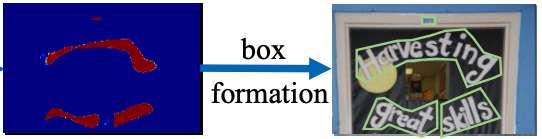
\includegraphics[width=0.45\textwidth]{img/STD-representation-curved-binary-Liao-Real-2019.png}}
    \subfigure[
        \scriptsize Textfield with vectors to text center
        \citep{xu_textfield_2019}\label{fig:curved-rep-xu-textfield-2019}
    ]{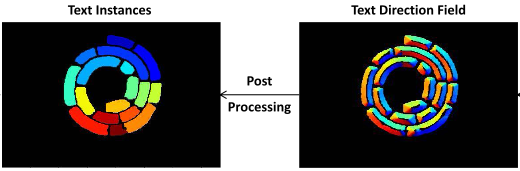
\includegraphics[width=0.45\textwidth]{%
        img/STD-representation-curved-textfield-Xu-textfield-2019.png}
    }
    \subfigure[
        \scriptsize Segmentation scales for label building
        \citep{wang_shape_2019}\label{fig:curved-rep-wang-shape-2019}
    ]{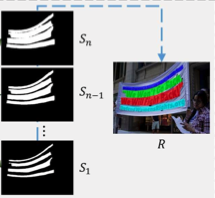
\includegraphics[width=0.25\textwidth]{img/STD-representation-curved-scale-Wang-Shape-2019.png}}
    \subfigure[
        \scriptsize Textsnake representation with centerline interconnected circles
        \citep{ferrari_textsnake_2018}\label{fig:curved-rep-ferarri-textsnake-2018}
    ]{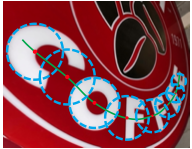
\includegraphics[width=0.30\textwidth]{%
        img/STD-representation-curved-textsnake-ferarri-textsnake-2018.png}
    }
    \caption{%
        Different curved text instance representation\label{fig:curved-text-representations}
    }
\end{figure}
The following approaches are concerned with performance for curved text:
A new representation for curved text was introduced
by~\cite{xu_textfield_2019} (see Figure~\ref{fig:curved-rep-xu-textfield-2019}).
The representation is made up of direction vectors that point away from the nearest border.
These vectors are predicted by magnitude and direction~\citep{xu_textfield_2019}.
The resulting text direction field can then be use to reconstruct text
instance~\citep{xu_textfield_2019}.
Another approach that improves text representation was introduced by~\cite{ferrari_textsnake_2018}.
The pixel level segmentation approach predicts the values that can be used to form the text
representation shown in Figure~\ref{fig:curved-rep-ferarri-textsnake-2018}.
The representation combins circles with a line to form a curved text
instance~\citep{ferrari_textsnake_2018}.
Another way of distinguishing between text instances is to progressively predict larger scale text
areas~\citep{wang_shape_2019} (see Figure~\ref{fig:curved-rep-wang-shape-2019}).
This is achieved by continuously shrinking the image with the help of
kernels~\citep{wang_shape_2019}.
This helps as the network can recognize at which scale the instances overlap~\citep{wang_shape_2019}.
Recent research has brought up approaches that use both segmentation and \ac{BB} regression in the
same architecture~\citep{xie_scene_2018,dai_fused_2018}.
The approach introduced by~\cite{xie_scene_2018} leverages text segmentation to rescore certainty
for predicted \acp{ROI} to improve \ac{NMS}, the filtered \acp{ROI} are then used to refine
\acp{BB} regression and text classification~\citep{xie_scene_2018}.
The innovation by~\cite{dai_fused_2018} improves feature extraction for \ac{STD} by fusing lower
level features.
These features are used for \ac{ROI} proposals and are then used to pool the fused feates for
the text/non-text classification, \ac{BB} regression and text segmentation
branches~\citep{dai_fused_2018}.
Similar to the previous approach, \ac{NMS} is modified to use a text segmentation map to better
work with curved text instance~\citep{dai_fused_2018,xie_scene_2018}.

\subsection{Recognition Innovations}
For \ac{STR} the search led to 8 results (see Table~\ref{tb:STR-steps-properties}).
The last relevant innovation was found on page 13 and at page 18 the search was stopped because
the results started to diverge.
The investigation of citations did not lead to new results.
\begin{table}[h]
    \centering\scriptsize
    \begin{tabular}{p{.09\textwidth}p{.16\textwidth}p{.192\textwidth}p{0.03\textwidth}
            p{0.3\textwidth}p{.05\textwidth}p{.05\textwidth}}
        \multicolumn{2}{c}{Approach category} & Source & \#cit & Innovation & Lexi-con & Stage \\
        \toprule
        Seg based & &~\cite{liao_scene_2018} & 120 & Combine different levels of character attention
            to localize characters and improve receptive fields with deformable convolution & w/o \\
        \midrule
        \ac{EnDe} based & & & \\
            & CTC based &~--- & & \\
            & Attention based &~\cite{zhan_esir_2019} & 181 & Iterative rectification with line fitting
                transformation & b & r \\
            & &~\cite{luo_multi-object_2019} & 174 & Rectification by removing character offset &
                b & r \\
            & &~\cite{shi_aster_2019} & 349 & Rectification based on grids & b & r \\
            & &~\cite{cheng_aon_2018} & 209 & Extract and combine character features in four directions
                & b & f \\
            & &~\cite{li_show_2019} & 141 & Simple pipeline combined with 2d attention mechanism
                & b & s\\
            & &~\cite{liu_char-net_2018} & 112 & Adapted attention mechanism to find
                individual characters and rectify local features for the decoder & b & s \\
            & &~\cite{bai_edit_2018} & 100 & Edit operations (consumption, deletion, insertion)
                influence probability of prediction & b & d \\
        \bottomrule
    \end{tabular}
    \captionsetup{justification=centering}
    \caption[Notable innovations for STR model architecture]{%
        Notable innovations for STR model architecture; \\
        w/: with lexicon, w/o: without lexicon, b: both; \\
        r: rectification, f: feature extraction, s: sequence modelling,
        d: decoding\label{tb:STR-steps-properties}
    }
\end{table}

The approach from~\cite{liao_scene_2018} works with localizing and classifying each character
separately~\citep{liao_scene_2018} which is why it fits into the segmentation based category.
The innovation leverages deformable convolution~\citep{dai_deformable_2017} to decide
which spatial information to focus on~\citep{liao_scene_2018}.
Additionally, it relies on a fully convolutional attention module which weakens background and
highlights characters at pixel level~\citep{liao_scene_2018}.
The attention module is performed at different scales~\citep{liao_scene_2018,xu_show_2016}.

The following approaches are all attention based, however their innovation concern different parts
of the attention based \ac{STR} pipeline.
The approaches by~\cite{zhan_esir_2019,luo_multi-object_2019,shi_aster_2019} all improve
text rectification ahead of the encoding step.
From~\cite{zhan_esir_2019} comes a rectification approach that iteratively estimates the fit of a
polynomyal to the text line and uses that prediction to rectify the text with \ac{TPS}
transformation~\citep{bookstein_principal_1989,zhan_esir_2019}.
Rectification is improved by~\cite{luo_multi-object_2019} by removing vertical offset of characters
to straighten the word out by placing a character lower or higher.
This works well for slanted images but has problems with curved text in contrast to the other
rectification modules~\citep{zhan_esir_2019,liu_star-net_2016,long_scene_2021}.
Fractional pickup is also introduced by~\cite{luo_multi-object_2019}.
It is a mechanism to improve the attention field of vision to lightly include adjacent characters
in order to improve robustness~\citep{luo_multi-object_2019}.
\begin{figure}[hb]
    \centering\scriptsize
    \subfigure[
        \scriptsize center line rectification
        \citep{zhan_esir_2019}\label{fig:rectification-zhan-esir-2019}
    ]{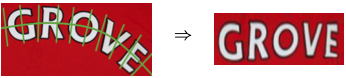
\includegraphics[width=0.35\textwidth]{img/STR-rectification-Zhan-ESIR-2019.png}}
    \subfigure[
        \scriptsize offset rectification
        \citep{luo_multi-object_2019}\label{fig:rectification-luo-multi-2019}
    ]{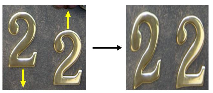
\includegraphics[width=0.20\textwidth]{img/STR-rectification-Luo-Multi-2019.png}}
    \subfigure[
        \scriptsize grid rectification
        \citep{shi_aster_2019}\label{fig:rectification-shi-aster-2019}
    ]{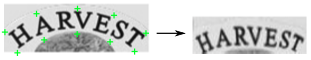
\includegraphics[width=0.35\textwidth]{img/STR-rectification-Shi-Aster-2019.png}}
    \caption{%
        Visualization of different innovations regarding
        rectification\label{fig:rectification-examples}
    }
\end{figure}
Similar to~\cite{zhan_esir_2019},~\cite{shi_aster_2019} estimates the text form by localizing
grid controlpoints that surround the text instance from the top and bottom.
The grid can then be used in conjunction with \acp{TPS}~\citep{shi_aster_2019}.

The approach by~\cite{cheng_aon_2018} improves features by extracting features for text in
four directions (right, up, left, down)~\citep{cheng_aon_2018}.
The feature vectors are then used with the other extracted features to act as a gate (similar to
\acp{LSTM})~\citep{cheng_aon_2018}.

\begin{figure}[ht]
    \centering\scriptsize
    \subfigure[
        \scriptsize 2d attention
        \citep{li_show_2019}\label{fig:2d-attention-li-show-2019}
    ]{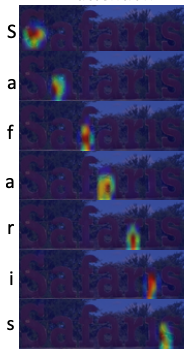
\includegraphics[width=0.20\textwidth]{img/STR-2d-attention-Li-Show-2019.png}}
    \subfigure[
        \scriptsize attention character rectification
        \citep{liu_char-net_2018}\label{fig:attention-rectification-liu-char-net-2018}
    ]{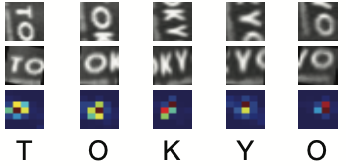
\includegraphics[width=0.55\textwidth]{img/STR-attention-rectification-Liu-Char-Net-2018.png}}
    \caption{%
        Effects of innovative attention mechanisms for STR\label{fig:attention-examples}
    }
\end{figure}
The next two approaches~\citep{li_show_2019,liu_char-net_2018} improve upon the attention mechanism
sequence modelling for \ac{STR}.
The innovation by~\cite{li_show_2019} uses 2d-attention from~\citep{xu_show_2016} to use
for \ac{STR}.
Additionally, the mechanism is made more robust by taking each of the eight spatial neighbors into
account~\citep{li_show_2019}.
The mechanism proposed by~\cite{liu_char-net_2018} uses attention to recurrently find characters and
\ac{TPS} to rectify them in order predict the text intance.
For each character, the corresponding feature region is extracted and is
rectified using a local spatial transformer~\citep{liu_char-net_2018}.
The last relevant \ac{STR} innovation improves upon the decoding and prediction process.

The approach from~\cite{bai_edit_2018} introduces the concept of edit probibilities.
At each state, the decoder decides which edit operation to perform (consumption, deletion, insertion)
based on their edit probibilities~\citep{bai_edit_2018}.
These operations either forego a time step, add a character to the word or insert a missed character
at the previous position~\citep{bai_edit_2018}.

\subsection{Spotting Innovations}
For end to end \ac{STS} 5 results where identified as relevant under the defined criteria.
The last relevant innovation was found on page 5 and at page 10 the topic diverged.
The investigation of citations did not lead to new results.
\begin{table}[h]
    \centering\scriptsize
    \begin{tabular}{p{.09\textwidth}p{.19\textwidth}p{0.03\textwidth}p{0.37\textwidth}
            p{0.07\textwidth}p{0.07\textwidth}}
    \textbf{Category} & \textbf{Source} & \textbf{\#cit} & \textbf{Innovation} &
                                        \textbf{Orien-tation} & \textbf{Lexi-con} \\
        \toprule
        2 step &~\cite{liao_textboxes_2018} & 499 & Combine Texboxes++ detection with \ac{CTC}
            recognition, used recognition confidence score for & m & b\\
            &~\cite{shi_aster_2019} & 349 & Textboxes++ \ac{BB} rectification and grid usage for
                attention recognition & c & b \\
        2 stage &~\cite{lyu_mask_2018} & 362 & \ac{ROI} detection followed by pixel and character
            segmentation & c & w/o \\
            &~\cite{liu_fots_2018} & 355 & Bilinear interpolation to transform oriented feature
                regions into axis-aligned feature maps followed by \ac{CTC} recognition
                & m & b \\
            &~\cite{liu_abcnet_2020} & 100 & One stage with bezier curves instead of anchor fee
                detection followed by bezier adjusted ROI pooling and a lightweight \ac{CTC}
                recognition head & c & b  \\
        \bottomrule
    \end{tabular}
    \captionsetup{justification=centering}
    \caption[Notable innovations for STS model architecture]{%
        Notable innovations for STS model architecture; \\
        c:curved, m:multi-oriented, h:horizontal; \\
        w/: with lexicon, w/o: without lexicon, b: both\label{tb:E2E-steps-properties}
    }
\end{table}

The listed two step approaches are not the innovations of the respective methods but rather a
a way to extend the proposed \ac{STD}/\ac{STR} to a \ac{STS}
solution~\citep{liao_textboxes_2018,shi_aster_2019}.
The \ac{STD} approach from~\cite{liao_textboxes_2018} can be extended with the \ac{CTC} based
approach from~\cite{shi_end--end_2017} which was explained along the taxonomy.
The word probability that is predicted by the \ac{CTC} transcription can be combined with the
text certainty score of the \ac{STD} module to improve \ac{NMS}.
The \ac{STR} approach from~\cite{shi_aster_2019} can be extended with the one stage
\ac{BB} regression based \ac{STD} approach from~\cite{liao_textboxes_2017} that was also explained
in the taxonomy~\citep{shi_aster_2019}.
\begin{figure}[ht]
    \centering
    \subfigure[
        \scriptsize STS architecture with feature sharing
        \citep{liu_fots_2018}\label{fig:attention-rectification-liu-char-net-2018}
    ]{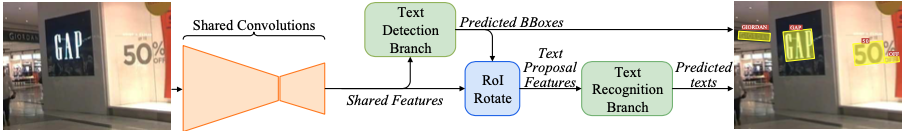
\includegraphics[width=0.8\textwidth]{img/E2E-2-stage-example-Liu-Fots-2018.png}}
    \subfigure[
        \scriptsize Rotated to axis aligned sampling effect
        \citep{liu_fots_2018}\label{fig:2d-attention-li-show-2019}
    ]{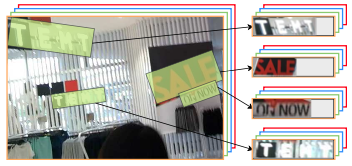
\includegraphics[width=0.40\textwidth]{img/E2E-2-stage-sampling-example-Liu-Fots-2018.png}}
    \caption[STS architecture with feature sharing]{%
        STS architecture with feature sharing and sampling
        effect~\citep{liu_fots_2018}\label{fig:2-stage-example-LIU-Fots-2018}
    }
\end{figure}

The field of end to end \ac{STS} has moved towards 2 stage approaches that combin both \ac{STD}
and \ac{STR}~\citep{lyu_mask_2018,long_scene_2021}.
The innovation from~\cite{liu_fots_2018} combines a oriented detection with combined pixel
segmentation and \acp{BB} with recognition by using bilinear interpolation to smaple and rotate
the spatial features corresponding to a text instance to be axis aligned~\citep{liu_fots_2018}.
The subsequent recognition branch is \ac{CTC} based.
The 2 stage approach introduced by~\cite{lyu_mask_2018} uses uses a \ac{RPN} to propose \acp{ROI}
which are used to extract features for both a \ac{BB} regression branch and a segmentation branch
which predicts text instances and characters on a pixel level~\citep{lyu_mask_2018}.
The \acp{BB} are used with the text instance segmentation to form the final detection prediction and
the characters are combined to the recognition prediction~\citep{lyu_mask_2018}.
The network from~\cite{liu_abcnet_2020} uses bezier curves for a new representation for curved text.
The bezier curve representation is predicted by a one stage, anchor free
regression~\citep{liu_abcnet_2020}.
The spatial features corresponding to the predicted instances are then extracted from the feature
maps and handed to a lightweight \ac{CTC} based recognition branch~\citep{lyu_mask_2018}.
